\documentclass[conference]{IEEEtran}

\IEEEoverridecommandlockouts

\usepackage{cite}
\usepackage{amsmath,amssymb}
\usepackage{graphicx}
\usepackage{booktabs}
\usepackage{array}
\usepackage{tabularx}
\usepackage{url}
\usepackage{xurl}
\usepackage{enumitem}
\usepackage{ragged2e}

\graphicspath{{../latex_report/figures/}}
\newcolumntype{Y}{>{\RaggedRight\arraybackslash}X}
\setlist[itemize]{leftmargin=*,nosep}
\setlist[enumerate]{leftmargin=*,nosep}
\renewcommand{\arraystretch}{1.12}
\newcounter{algorithm}

\begin{document}

\title{An Explainable and Cost-Efficient AI Resume Screening Framework Using OCR-Aware Parsing, TF-IDF Similarity, and Bounded Weighted Scoring}

\author{
\IEEEauthorblockN{Rohan Garg}
\IEEEauthorblockA{\textit{Department of Computer Science and Engineering}\\
\textit{Delhi Technological University}\\
New Delhi, India\\
2K22/CO/375}
\and
\IEEEauthorblockN{Punit Sukhani}
\IEEEauthorblockA{\textit{Department of Computer Science and Engineering}\\
\textit{Delhi Technological University}\\
New Delhi, India\\
2K22/CO/353}
\and
\IEEEauthorblockN{Saksham}
\IEEEauthorblockA{\textit{Department of Computer Science and Engineering}\\
\textit{Delhi Technological University}\\
New Delhi, India\\
2K22/CO/395}
}

\maketitle

\begin{abstract}
The first stage of recruitment is increasingly mediated by automated resume screening systems. However, many available systems occupy two unsatisfactory extremes: simple keyword filters are fast but brittle, while transformer-based or large language model approaches provide richer semantic matching at higher computational cost and with reduced transparency. This paper presents a lightweight, explainable, and OCR-aware resume screening framework for first-pass candidate ranking. The proposed system accepts resumes in heterogeneous formats, normalizes text through digital parsing and optical character recognition fallback, extracts technical skills, soft skills, and years of experience through a rule-guided natural language processing layer, computes contextual relevance through TF-IDF cosine similarity, and produces a bounded weighted score with plain-language explanations. The framework is implemented as a modular Flask-based application with a recruiter-facing dashboard for weight configuration and score inspection. Five benchmarks evaluate format-bias resilience, keyword-stuffing resistance, mathematical boundary handling, lexical-versus-semantic trade-offs, and batch efficiency. Results show that the proposed Regex+TF-IDF architecture processes 100 resumes in 0.0062 seconds with 0.12 MB peak memory in the measured benchmark, while a Sentence-BERT baseline requires 4.1860 seconds and 7.33 MB. The system is not intended to replace human hiring judgment or deep semantic evaluation, but it provides a practical, auditable, and low-cost first-pass screening layer for small and medium-sized organizations.
\end{abstract}

\begin{IEEEkeywords}
resume screening, applicant tracking system, explainable AI, TF-IDF, OCR, recruitment automation, cosine similarity, natural language processing
\end{IEEEkeywords}

\section{Introduction}
Digital recruitment has significantly increased the number of applications received for a single job posting. Online job portals allow applicants to apply across locations with very low effort, and organizations often receive hundreds or thousands of resumes for a single opening. Human recruiters therefore spend substantial time performing repetitive first-stage screening. This stage is also vulnerable to inconsistency because reviewers may give excessive weight to formatting, university names, familiar employers, or visually prominent sections rather than the actual match between candidate capabilities and role requirements \cite{b3}, \cite{b10}.

Applicant Tracking Systems (ATS) were introduced to reduce this workload, but many traditional systems operate primarily through rigid keyword matching. A job description requiring ``Python'', ``REST'', and ``PostgreSQL'' may cause the system to search for these exact terms in candidate resumes. This approach is computationally inexpensive, but it creates false negatives when a candidate uses alternate wording, abbreviations, or semantically related phrasing. It is also vulnerable to keyword stuffing, where candidates insert repeated job-description terms into resumes in order to inflate match scores.

Recent recruitment systems increasingly use transformer-based semantic embeddings and large language models. These methods can map related expressions such as ``RESTful APIs'' and ``REST'' into nearby semantic spaces, reducing lexical brittleness \cite{b6}, \cite{b12}. However, they introduce two practical challenges. First, they increase latency, memory consumption, and deployment cost, particularly when processing large batches. Second, they often behave as black-box scoring layers. A recruiter may receive a high or low match score without a clear, auditable explanation of which job requirements were satisfied, missing, or over-weighted. In hiring contexts, such opacity is not merely inconvenient; it can reduce trust and make candidate rejection decisions difficult to justify \cite{b8}, \cite{b14}.

This paper presents a practical middle-ground architecture for first-pass resume screening. The proposed framework combines deterministic skill extraction, TF-IDF cosine similarity, bounded weighted scoring, optical character recognition fallback, and rule-based explainability. Rather than claiming complete semantic understanding, the framework is designed around three constraints common in small and medium-sized enterprise recruitment: speed, low deployment cost, and auditability. The system ranks candidates according to technical skill coverage, soft skill evidence, years of experience, contextual similarity, and capped extra-skill bonuses. Each score is converted into a plain-language explanation that lists matched skills, missing skills, detected soft skills, experience fit, and bonus skills.

The main contributions of this work are:
\begin{itemize}
    \item an end-to-end OCR-aware resume screening pipeline that handles text, PDF, and image resumes using digital extraction followed by OCR fallback;
    \item a bounded weighted scoring model that combines technical skills, soft skills, experience, contextual similarity, and capped extra-skill bonuses;
    \item an explainable AI layer that converts score components into recruiter-readable justifications;
    \item a benchmark-driven comparison of the lightweight Regex+TF-IDF design against semantic embedding alternatives with respect to robustness, efficiency, and interpretability.
\end{itemize}

\section{Related Work}
\subsection{Keyword-Based Resume Screening}
Early ATS solutions used Boolean search and keyword frequency counts to match resumes against job descriptions. Such systems are simple to implement and can process large document batches quickly \cite{b1}, \cite{b3}. Their weakness is that they treat language as exact strings. A candidate who writes ``backend service development'' may be relevant to a backend engineering role, but a strict keyword system may not reward that expression unless it contains the exact expected keywords. Rigid matching also encourages applicant behavior that optimizes for the parser rather than for truthful skill representation.

\subsection{Classical NLP and Vector-Space Models}
Classical machine learning methods provide a middle layer between exact keyword search and deep semantic modeling. TF-IDF assigns greater importance to terms that are frequent in a document but not common across the corpus. When used with cosine similarity, it provides a fast numerical estimate of textual relevance \cite{b7}, \cite{b10}. In resume screening, TF-IDF is useful because it reduces the influence of generic terms and can penalize verbose, unrelated content. Rule-guided NLP can complement TF-IDF by extracting structured attributes such as skills and years of experience \cite{b16}.

\subsection{Transformer-Based Semantic Matching}
Transformer-based models such as BERT and Sentence-BERT improve semantic matching by embedding sentences into vector spaces where related meanings can be compared \cite{b6}, \cite{b12}. Recent recruitment systems use such embeddings, LLM feedback loops, and multi-agent frameworks to match candidate profiles and job descriptions more flexibly \cite{b2}, \cite{b5}, \cite{b11}, \cite{b13}. These models are valuable when candidates and recruiters use different vocabulary for the same competence. However, they demand more memory and computation than lexical approaches, and they may not naturally produce explanations that are easy for non-technical HR users to audit.

\subsection{Explainable AI in Recruitment}
Explainable AI is especially important in hiring because ranking decisions can affect career opportunities \cite{b8}, \cite{b14}. General-purpose methods such as SHAP and LIME can help analyze complex models, but their outputs may be too technical for everyday recruitment workflows \cite{b9}. A recruiter usually needs concrete statements such as ``matched two out of four required skills'' or ``missing PostgreSQL and REST'', not only feature-attribution plots. The present system therefore uses a rule-based explanation layer aligned with the internal score dictionary.

\subsection{Format Bias and OCR-Based Parsing}
Resume screening systems can unintentionally penalize candidates because of file format rather than content. A parser may fail on scanned PDFs, image resumes, or visually designed resumes with non-linear layouts \cite{b7}, \cite{b15}. OCR fallback reduces such format bias by recovering text when native extraction fails. Although OCR can introduce character-level noise, image preprocessing such as grayscale conversion, binarization, and sharpening can improve extraction quality for standard resume images.

\section{Problem Formulation}
Let \(R=\{r_1,r_2,\ldots,r_n\}\) be a batch of resumes submitted for a job description \(J\). The objective is to produce a ranked list \(L\) where each candidate receives a bounded match score \(S_i \in [0,100]\) and an explanation \(E_i\). The system must satisfy four operational requirements.

First, the system should accept multiple document formats and reduce parser-induced discrimination. Second, it should reward explicit required skills while resisting naive keyword stuffing. Third, the scoring model should remain computationally inexpensive enough for batch execution on ordinary hardware. Fourth, the recruiter should be able to inspect why a candidate was ranked high or low.

The screening task is therefore formulated not as a fully autonomous hiring decision, but as an auditable first-pass filtering problem:
\begin{equation}
f(r_i,J,W) \rightarrow (S_i,E_i),
\end{equation}
where \(W\) denotes recruiter-configurable scoring weights. The final ranked list is obtained by sorting all \((S_i,E_i)\) pairs in descending score order.

\subsection{Design Objectives}
The proposed framework was designed around five objectives derived from practical recruitment workflows.

\textit{O1: Format tolerance.} A candidate should not be disadvantaged only because the resume is submitted as an image, scanned PDF, or digital document with imperfect text extraction. The system therefore includes a fallback path rather than assuming that every resume is clean text.

\textit{O2: Bounded scoring.} Every component must have a clear mathematical upper bound. This prevents over-qualified candidates, keyword-stuffed resumes, or long skill lists from breaking the final scoring range.

\textit{O3: Low computational cost.} The first-pass screening layer should operate on commodity hardware without requiring cloud GPU instances or paid model APIs. This makes the system suitable for academic prototypes and small organizations.

\textit{O4: Recruiter interpretability.} A score must be accompanied by a direct explanation. The explanation should be understandable without requiring knowledge of embedding spaces, probability calibration, or model attribution algorithms.

\textit{O5: Human-in-the-loop decision support.} The system should rank and explain candidates, but it should not make final hiring decisions. The output is designed to support recruiter prioritization and further review.

\subsection{Data Representation}
Each processed resume is represented internally as a structured record. The record contains the original file name, extracted raw text, normalized text, detected technical skills, detected soft skills, inferred years of experience, contextual similarity, component scores, final score, and natural-language explanation. This structure allows the system to separate evidence extraction from ranking. If the scoring formula is changed, the same extracted evidence can be re-weighted without reparsing the original document.

The job description is represented similarly, but its extracted fields act as requirements rather than candidate attributes. For example, if the job description contains Python, Django, PostgreSQL, and REST, these are treated as required technical terms. If the job description specifies three years of experience, that value becomes the denominator for the bounded experience score. The separation of resume evidence and job requirements keeps the method explicit and auditable.

\subsection{Scope of Automation}
The proposed framework deliberately avoids sensitive demographic inference. It does not attempt to infer gender, caste, religion, ethnicity, age, photograph attributes, or personal background. Its ranking features are restricted to text-derived role relevance: skills, experience, and contextual job-description similarity. This does not by itself guarantee full fairness, but it reduces the risk of directly encoding protected attributes into the scoring pipeline.

\section{System Architecture}
The proposed architecture is organized into five modules: document parsing, NLP extraction, weighted matching, explainable AI, and visualization. Fig.~\ref{fig:architecture} presents the overall flow from uploaded resumes and job description to ranked output.

\begin{figure*}[t]
    \centering
    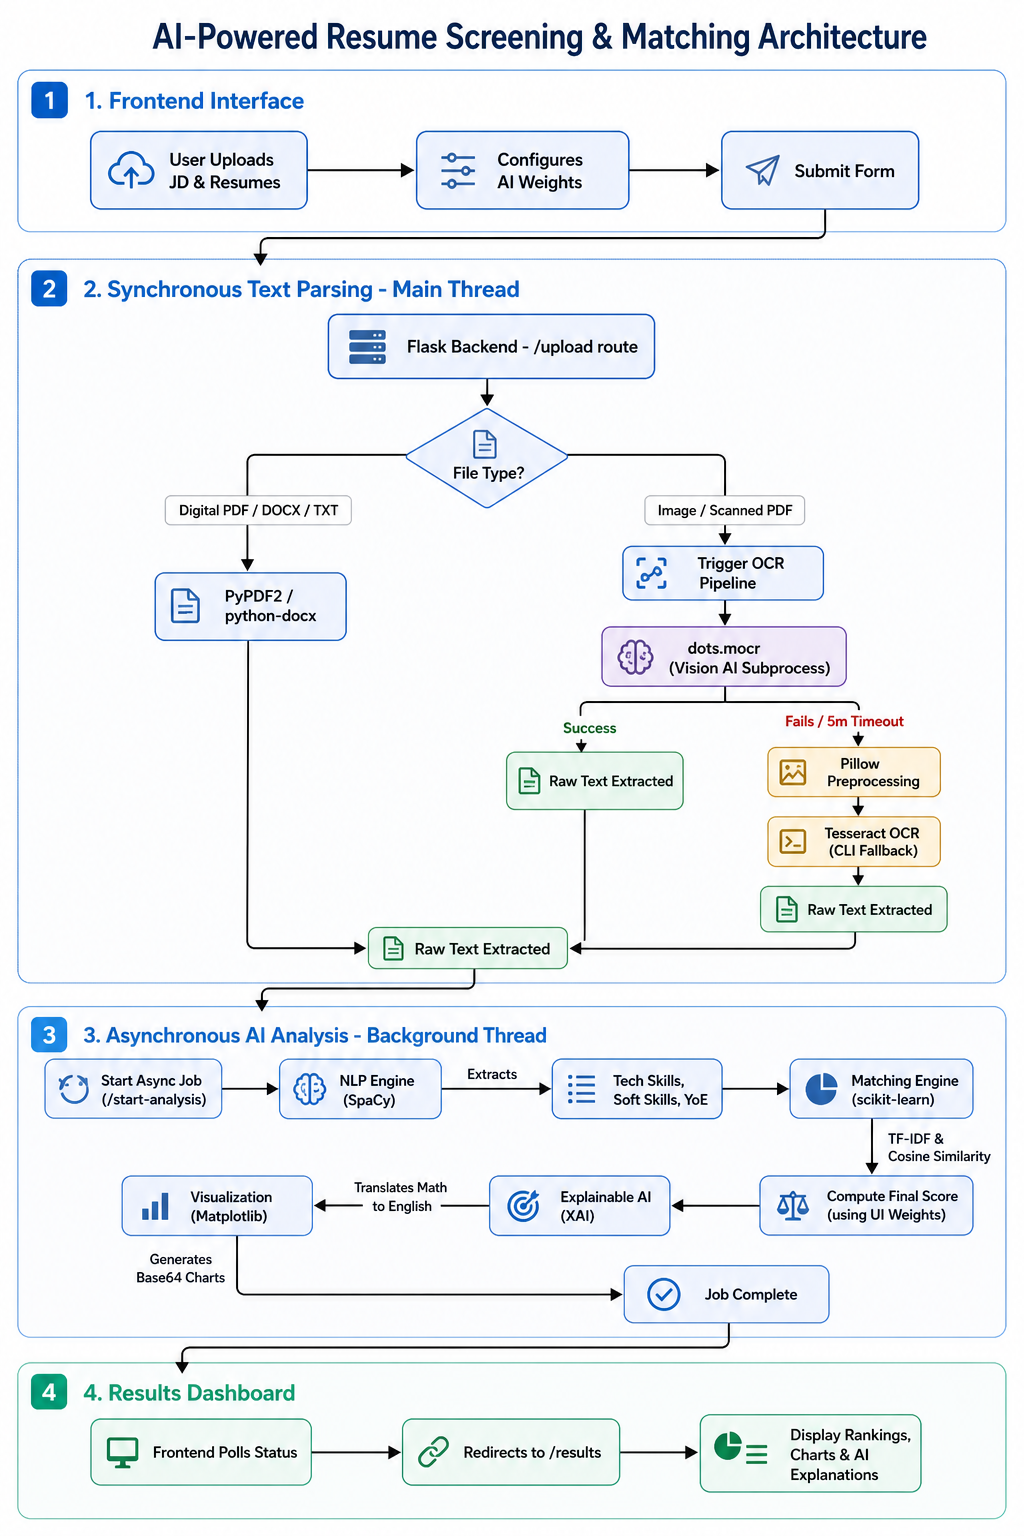
\includegraphics[width=0.86\textwidth]{project_flowchart.png}
    \caption{End-to-end architecture of the proposed AI-powered resume screening system.}
    \label{fig:architecture}
\end{figure*}

\subsection{Document Parsing Layer}
The parsing layer receives resumes in text, PDF, Word, or image formats. Native text is read directly. Digital PDF files are processed through PDF text extraction. Word files are parsed through the document XML structure. If extracted text is below a minimum threshold, the document is treated as scanned or parser-resistant and routed to OCR. Image resumes are directly routed to the OCR path.

\subsection{OCR Fallback Layer}
The OCR fallback layer applies image preprocessing before character recognition. In the implemented parser, image-based resumes and scanned PDFs are first routed through the available dots.mocr provider. If that provider fails or is disabled, the system falls back to the Tesseract command-line engine. Before Tesseract execution, transparent images are flattened onto a white background, converted to grayscale, contrast-enhanced, sharpened, and binarized using a fixed intensity threshold. For scanned PDFs, pages are converted to 300 DPI images before OCR. This fallback is intended to prevent candidates from being penalized simply because their resumes are scanned or image-based.

\subsection{NLP Extraction Layer}
The normalized text is lowercased and processed by a lightweight NLP module. SpaCy's \texttt{en\_core\_web\_sm} model is used for tokenization, lemmatization, stop-word filtering, and named-entity extraction. Technical and soft skills are not extracted through generic NER; they are matched using strict regular-expression word boundaries against curated skill lists. This is done to avoid false positives such as matching a single-letter technical skill inside an unrelated word. The technical list includes terms such as Python, Django, REST, Docker, AWS, PostgreSQL, and related technologies, while the soft-skill list includes terms such as leadership, communication, collaboration, and cross-functional work. Regular expressions identify direct and indirect years-of-experience evidence such as ``5 years of experience'', ``experience: 5 years'', and date ranges.

\subsection{Matching and Ranking Layer}
The matching layer computes four principal components: technical skill score, soft skill score, years-of-experience score, and contextual similarity. Technical and soft scores are based on coverage of required skills. Experience is capped so that over-qualified candidates do not receive more than the maximum allotted experience weight. Contextual similarity is calculated using TF-IDF vectors and cosine similarity.

\subsection{Explainable AI Layer}
The explanation layer receives the internal score dictionary and converts it into plain-language justification. Rather than post-hoc approximating a black-box model, it directly reports the exact symbolic components used in scoring. This produces statements listing matched required skills, missing skills, detected extra skills, experience fit, and score contribution by component.

\subsection{Module Responsibilities}
Table~\ref{tab:modules} summarizes the responsibility of each module. This decomposition is important because recruitment screening combines document engineering, NLP, mathematical scoring, and user-interface concerns. Keeping these functions separate improves maintainability and allows individual modules to be replaced later.

\begin{table*}[t]
\centering
\caption{Functional Responsibilities of the Proposed Framework}
\label{tab:modules}
\small
\begin{tabularx}{\textwidth}{p{0.18\textwidth}p{0.25\textwidth}Y}
\toprule
\textbf{Module} & \textbf{Input and Output} & \textbf{Responsibility}\\
\midrule
Document parser & File stream \(\rightarrow\) raw text & Reads digital documents, detects low-quality extraction, and routes scanned or image-based resumes to OCR fallback.\\
OCR fallback & Image representation \(\rightarrow\) recovered text & Applies preprocessing and optical character recognition to reduce format bias for non-searchable resumes.\\
NLP extractor & Normalized text \(\rightarrow\) structured attributes & Uses SpaCy for linguistic preprocessing and NER, while detecting technical skills, soft skills, and years of experience through curated dictionaries and regular expressions.\\
Matching engine & Resume attributes and JD attributes \(\rightarrow\) score dictionary & Computes technical coverage, soft-skill coverage, experience score, TF-IDF context score, bonus score, and final score.\\
XAI generator & Score dictionary \(\rightarrow\) explanation & Produces recruiter-readable explanations containing matched, missing, and extra skills along with score components.\\
Dashboard & Ranked JSON records \(\rightarrow\) visual interface & Displays configurable weights, ranked candidates, score breakdowns, and explanation panels.\\
\bottomrule
\end{tabularx}
\end{table*}

\section{Proposed Methodology}
\subsection{End-to-End Screening Algorithm}
The complete workflow is shown in Algorithm~\ref{alg:endtoend}. This algorithm is included explicitly because the project is best understood as a step-wise transformation from raw input files to ranked recruiter-facing output.

\begin{figure*}[t]
\hrule
\vspace{3pt}
\refstepcounter{algorithm}\label{alg:endtoend}
\textbf{Algorithm~\thealgorithm: OCR-Aware Explainable Resume Screening Pipeline}
\vspace{3pt}
\hrule
\vspace{4pt}
\begin{enumerate}
    \item \textbf{Input:} Resume batch \(R\), job description \(J\), scoring weights \(W=(W_t,W_s,W_e,W_c)\), bonus cap \(B_{max}\).
    \item Parse \(J\) and extract required technical skills, soft skills, and required experience.
    \item For each resume \(r_i \in R\):
    \begin{enumerate}
        \item Detect file type of \(r_i\).
        \item If the file is native text or a digital document, perform digital text extraction.
        \item If extracted text length is below threshold \(\tau\), convert the file to image representation and invoke OCR fallback.
        \item If the file is an image, apply OCR using the available OCR provider; if Tesseract fallback is required, flatten transparency, convert to grayscale, boost contrast, sharpen, binarize, and run OCR.
        \item Normalize extracted text by lowercasing, removing noisy tokens, and standardizing spacing.
        \item Extract candidate technical skills, soft skills, and years of experience using skill ontology and regular expressions.
        \item Compute technical coverage, soft-skill coverage, capped experience match, and TF-IDF cosine similarity.
        \item Compute capped extra-skill bonus from skills present in resume but absent in the job description.
        \item Calculate final weighted score \(S_i\).
        \item Generate explanation \(E_i\) from matched, missing, bonus, and score-breakdown fields.
    \end{enumerate}
    \item Sort all candidate outputs by \(S_i\) in descending order.
    \item \textbf{Output:} Ranked candidate list \(L=\{(r_i,S_i,E_i)\}\) and dashboard visualizations.
\end{enumerate}
\vspace{2pt}
\hrule
\end{figure*}

\subsection{Parsing and OCR Thresholding}
The parser uses a threshold \(\tau=50\) characters to decide whether native PDF extraction is sufficient. If a PDF returns fewer than \(\tau\) characters, the system assumes that the document may be scanned, protected, or otherwise unsuitable for native text extraction. The parser also checks the PDF magic-byte header so that images renamed with a \texttt{.pdf} extension can be routed to image OCR instead of failing inside the PDF reader. This threshold is intentionally simple because the goal is robust first-pass routing rather than perfect document-layout reconstruction.

The thresholding strategy also reduces unnecessary OCR use. OCR is slower than direct text extraction, and applying it to every digital document would waste computation. The system therefore follows a preference order: native text extraction is attempted first, and OCR is used only when extraction confidence is low. In practical terms, this means that ordinary text resumes and searchable PDFs remain fast, while scanned documents still receive a recovery path.

\subsection{Text Normalization}
After extraction, the text is normalized before feature extraction. Normalization includes lowercasing and reducing repeated whitespace. The implementation intentionally preserves punctuation because technical tokens such as \texttt{C++}, \texttt{Node.js}, and experience ranges such as \texttt{1-3} can lose meaning if punctuation is removed aggressively. This step is necessary because different parsers produce different artifacts. For instance, PDF extraction may concatenate words that were visually separated, while OCR may introduce line breaks at unexpected positions. Although normalization cannot repair every artifact, it improves consistency across file types and reduces downstream extraction errors.

The system avoids aggressive stemming for technical skills because many technology names are meaningful in their original forms. For example, ``R'', ``REST'', ``React'', and ``Redis'' are distinct tokens and should not be collapsed carelessly. The extraction layer therefore prioritizes explicit skill dictionaries and carefully bounded regular expressions rather than broad morphological reduction.

\subsection{Skill and Experience Extraction}
Let \(T_J\) denote the set of technical skills required by the job description and \(T_R\) denote the set extracted from a resume. The technical skill score is:
\begin{equation}
S_{tech}=\frac{|T_J \cap T_R|}{|T_J|}\times 100.
\end{equation}
Similarly, if \(P_J\) is the set of requested soft skills and \(P_R\) is the set found in the resume, then:
\begin{equation}
S_{soft}=\frac{|P_J \cap P_R|}{|P_J|}\times 100.
\end{equation}
When a job description does not explicitly request soft skills, the soft component can be neutralized or assigned according to recruiter settings.

Skill extraction is performed using boundary-aware matching. A direct substring search can create false positives; for example, matching ``R'' inside ``manager'' would be incorrect. The extractor therefore treats skills as tokens or multi-word expressions with boundary conditions. For multi-word skills, the system searches normalized phrases. For single-token skills, the system checks surrounding boundaries to avoid accidental partial matches.

Soft skills are treated more cautiously than technical skills because they are often expressed indirectly. A candidate may demonstrate leadership through a phrase such as ``managed a team of six engineers'' even without writing the exact word ``leadership''. The current prototype detects explicit soft-skill terms, which keeps the method transparent but limits semantic recall. This is one reason why the future hybrid architecture is valuable.

Experience is treated as a bounded requirement. If \(Y_R\) is detected candidate experience and \(Y_J\) is required experience, the experience score is:
\begin{equation}
S_{exp}=\min\left(\frac{Y_R}{Y_J},1.0\right)\times 100.
\end{equation}
The cap prevents a candidate with double the required experience from receiving a mathematically inflated 200\% experience score.

\subsection{Contextual Similarity}
The system uses TF-IDF vectorization to represent the resume and job description as vectors. The primary implementation uses scikit-learn's \texttt{TfidfVectorizer} with English stop-word removal, a maximum vocabulary size of 5000, and unigram-plus-bigram features \((1,2)\). The bi-gram setting captures short technical phrases such as ``machine learning'' without loading a neural embedding model. Let \(A\) be the resume vector and \(B\) be the job-description vector. Their contextual similarity is computed by cosine similarity:
\begin{equation}
S_{ctx}=\frac{A \cdot B}{\|A\|\|B\|}\times 100.
\end{equation}
TF-IDF rewards distinctive terms more strongly than generic words. In combination with cosine normalization, it reduces the benefit of simply making a resume longer or repeatedly inserting a subset of terms, which is useful for resisting simple keyword-stuffing attacks.

\subsection{Bounded Weighted Score}
Recruiters may tune component weights before analysis. The default configuration used in the prototype is:
\begin{equation}
W_{tech}=0.60,\quad W_{soft}=0.10,\quad W_{exp}=0.15,\quad W_{ctx}=0.15,
\end{equation}
where:
\begin{equation}
W_{tech}+W_{soft}+W_{exp}+W_{ctx}=1.0.
\end{equation}
The final score is:
\begin{equation}
\begin{split}
S_{final}={}&(S_{tech}W_{tech})+(S_{soft}W_{soft})\\
&+(S_{exp}W_{exp})+(S_{ctx}W_{ctx})+B.
\end{split}
\end{equation}
The extra-skill bonus \(B\) is computed from skills that appear in the resume but are not explicitly required by the job:
\begin{equation}
B=\min\left(|T_R-T_J|\times \frac{B_{max}}{10},B_{max}\right).
\end{equation}
The cap prevents score inflation when candidates list many adjacent technologies.

\subsection{Explanation Template}
The explanation generator follows a deterministic template. For each candidate, it reports the match level, final score, experience status, matched required skills, missing required skills, extra technical skills, and score breakdown. A representative explanation has the following form:

\begin{quote}
Candidate \(X\) is a moderate match with a score of \(S\). The candidate meets the experience requirement \((Y_R/Y_J)\). They match \(m/k\) required technical skills: [matched list]. Missing skills are: [missing list]. Additional skills not in the job description are: [bonus list]. Score breakdown: technical, soft skills, experience, context, and bonus.
\end{quote}

This template is intentionally plain. A recruitment explanation should be immediately actionable. If the recruiter sees that a candidate is missing PostgreSQL and REST, the next review step is clear. The explanation also makes it easier to identify extraction errors. If a candidate obviously has a skill but the explanation lists it as missing, the recruiter can inspect the resume and update the skill ontology if required.

\subsection{Complexity Analysis}
Let \(n\) be the number of resumes, \(d\) the number of unique terms in the TF-IDF vocabulary for a comparison, and \(k\) the number of skills in the ontology. Digital parsing is approximately linear in document length. Skill matching is proportional to the number of ontology entries and the length of the normalized text, although practical implementations can optimize this through token sets and compiled regular expressions. TF-IDF vectorization is sparse and efficient for short documents such as resumes and job descriptions.

The most expensive branch is OCR, which depends on image resolution and preprocessing cost. However, OCR is only invoked for image files or failed digital extraction. This conditional design helps the system remain efficient for typical batches where many resumes are searchable PDFs or text documents. The final sorting step is \(O(n\log n)\), which is negligible compared with parsing and feature extraction for realistic resume batches.

\subsection{Why Not Use Only an LLM?}
A pure LLM or embedding-based system can improve semantic recall, but it changes the deployment profile. It introduces model loading time, increased memory, possible API dependency, prompt sensitivity, and explanation challenges. For a final hiring decision, semantic models may be useful. For the first screening layer, however, the system often needs to process large volumes quickly and produce deterministic reasons. The proposed design therefore prioritizes inexpensive ranking and explicit auditability. It also leaves room for future semantic modules as optional second-stage components rather than mandatory infrastructure.

\subsection{Feature Engineering Rationale}
The framework deliberately separates features into hard evidence and soft evidence. Hard evidence includes explicit technical skills and years of experience. These are treated as bounded requirements because many roles cannot ignore them. For example, if a backend role requires Django and PostgreSQL, a candidate lacking both should not be ranked highly only because the resume contains general software-engineering language. Soft evidence includes contextual similarity and soft-skill terms. These features help distinguish candidates with similar hard-skill coverage but should not overpower required competencies.

The extra-skill bonus is also separated from the base score. This distinction matters because additional skills can be useful but should not compensate completely for missing required skills. A candidate who knows Docker, Redis, and Kubernetes may be attractive for a backend role, but if the job explicitly requires PostgreSQL and the resume lacks it, the missing requirement should remain visible. The capped bonus captures adjacent value without hiding gaps.

\subsection{Score Band Interpretation}
For practical dashboard use, the final score can be mapped into qualitative bands. A high match indicates strong required-skill coverage and adequate experience. A medium match indicates partial alignment or missing secondary requirements. A partial match indicates that some relevant context exists but core requirements are missing. A low match indicates weak alignment with the job description. These bands are not used as automatic rejection labels; they are visual cues for prioritizing review.

The score bands are intentionally derived from the same score dictionary used for explanation. This avoids the inconsistency of a dashboard showing a candidate as ``high match'' while the explanation suggests major missing requirements. The recruiter can therefore move between the ranked list and the detailed explanation without encountering contradictory signals.

\section{Implementation}
The prototype was implemented as a modular Python web application. Flask provides the backend server and routing. The document parsing layer uses native file readers and OCR fallback. The NLP layer uses SpaCy tokenization, lemmatization, named-entity extraction, regular expressions, and curated skill dictionaries. The matching layer uses scikit-learn TF-IDF vectorization and cosine similarity. The dashboard is built using HTML, CSS, Bootstrap, Jinja2 templates, JavaScript, Matplotlib, and Chart.js.

\begin{table}[t]
\centering
\caption{Implementation Stack}
\label{tab:stack}
\small
\begin{tabularx}{\columnwidth}{p{0.30\columnwidth}Y}
\toprule
\textbf{Component} & \textbf{Technology and Purpose}\\
\midrule
Backend & Python and Flask for routing, upload handling, and session flow.\\
NLP & SpaCy tokenization, lemmatization, NER, regular expressions, and skill dictionaries for extraction.\\
Similarity & TF-IDF and cosine similarity for contextual matching.\\
Parsing & PyPDF2, python-docx, text reading, image parsing, dots.mocr/Tesseract OCR fallback, and PDF-to-image conversion for scanned documents.\\
Storage & SQLite, SQLAlchemy, Flask-Login, password hashing, and optional Google OAuth SSO for lightweight user/session persistence.\\
Frontend & Bootstrap, Jinja2, JavaScript, Matplotlib Base64 charts, and Chart.js for dashboards.\\
\bottomrule
\end{tabularx}
\end{table}

\subsection{Backend Flow}
When a recruiter uploads resumes and a job description, the backend receives a multipart request and stores uploaded content and weight settings server-side under a UUID key. Each resume is processed through the parser, NLP extractor, matcher, and explanation layer. Results are returned as structured objects containing candidate name, score components, matched skills, missing skills, bonus skills, detected soft skills, and generated explanation text. The dashboard then sorts the candidates from highest score to lowest score.

The backend design follows separation of concerns. The parser does not know how scores are calculated. The matcher does not know how files were uploaded. The explanation layer does not recompute evidence; it consumes the score dictionary generated by the matcher. This modularity makes the prototype easier to test. Individual benchmark scripts can target the parser, matching engine, or explanation generator without running the full web application.

\subsection{Concurrency and User Experience}
Batch resume screening can create long-running requests if all files are processed synchronously inside the main request-response cycle. The prototype therefore treats processing as a detached background task from the perspective of the user interface. The analysis page starts a daemon background thread and polls a status endpoint at regular intervals while the backend processes the uploaded batch. This avoids a frozen user interface and makes the application more usable for multi-resume uploads.

The dashboard is designed around recruiter workflow rather than model demonstration alone. A recruiter first configures weights, uploads the job description and resumes, waits for processing, and then reviews ranked results. For each candidate, the recruiter can inspect not only the final score but also the reason behind it. This supports quick triage while preserving transparency.

\subsection{Recruiter-Controlled Weighting}
The frontend provides controls for tuning the scoring weights before the run. In the implemented interface, four primary sliders share a normalized 100\% pool for technical skills, soft skills, experience, and context. A fifth bonus slider is isolated because the bonus is an additive capped offset rather than part of the normalized base score. This is important because different roles require different emphasis. A backend engineering role may prioritize technical coverage, while a project-management role may assign more weight to soft skills and experience. Fig.~\ref{fig:config} shows the scoring configuration interface.

\begin{figure}[t]
    \centering
    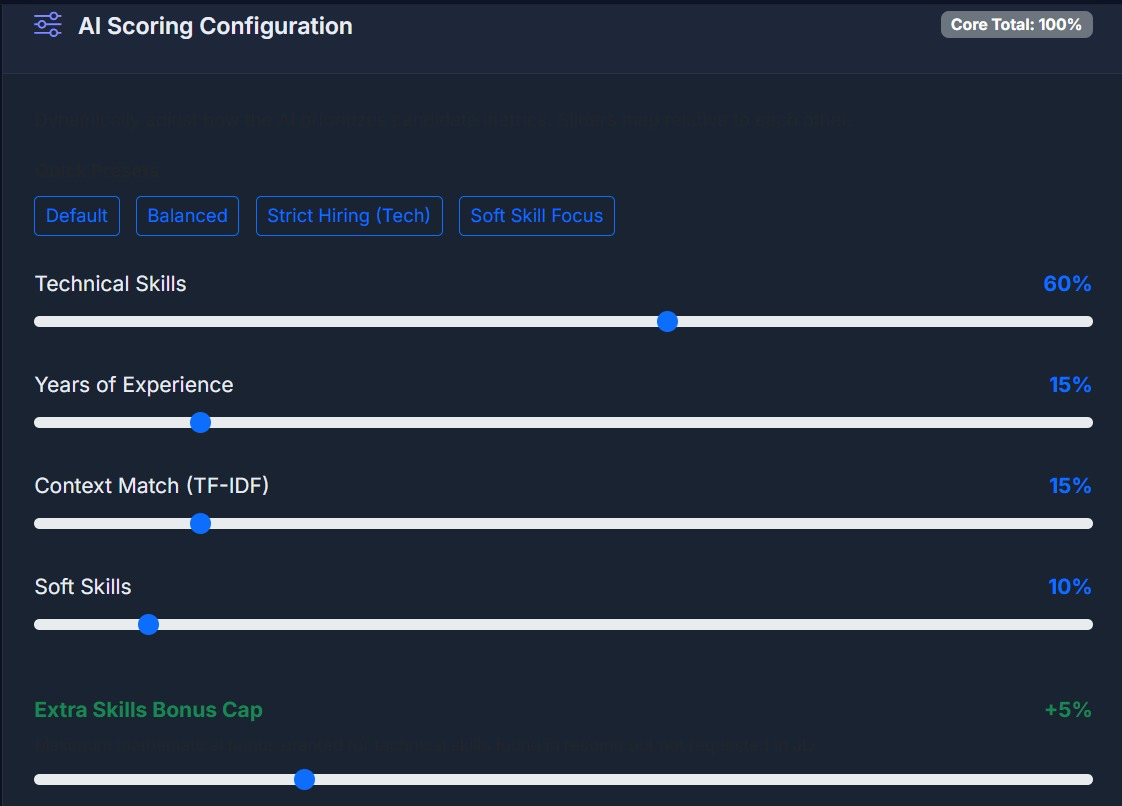
\includegraphics[width=\columnwidth]{ai_scoring_configuration.png}
    \caption{Recruiter-facing scoring configuration with adjustable weights.}
    \label{fig:config}
\end{figure}

\subsection{Explainable Output}
The result dashboard does not expose only a single final score. It decomposes the score into technical skills, soft skills, experience, context match, and bonus contribution. The expanded explanation panel lists matched and missing job-description skills, which makes the score traceable. Fig.~\ref{fig:xai} shows the explainable score breakdown interface.

\begin{figure}[t]
    \centering
    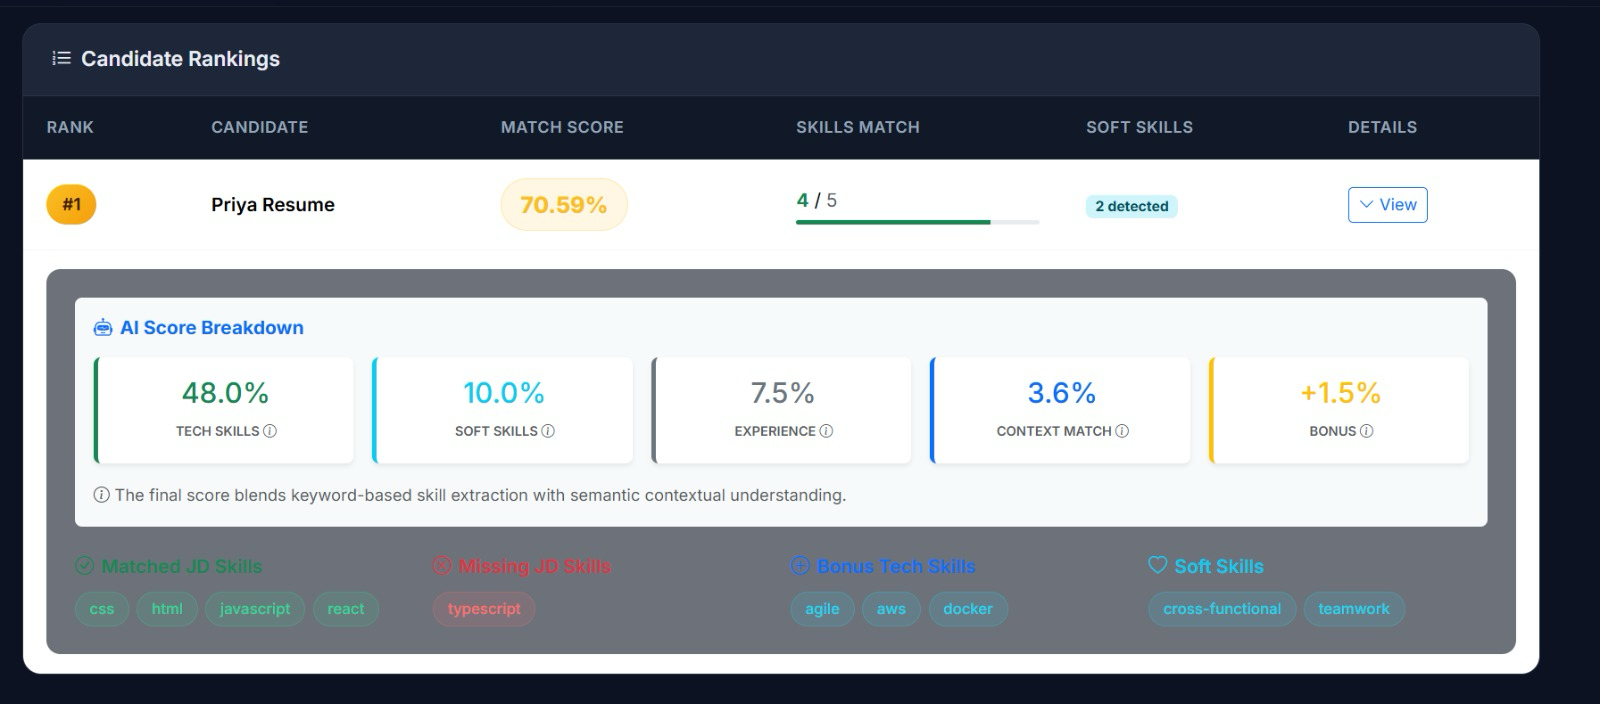
\includegraphics[width=\columnwidth]{ai_score_breakdown.png}
    \caption{Explainable AI score breakdown for recruiter auditability.}
    \label{fig:xai}
\end{figure}

\subsection{Illustrative Processing Case}
Consider a job description requiring Python, Django, PostgreSQL, and REST with three years of experience. A candidate resume states that the applicant has six years of backend development experience, mentions Python and Django, and lists AWS, Docker, Kubernetes, and Redis as additional technologies. The parser first extracts the resume text. The NLP layer identifies Python and Django as matched required skills, PostgreSQL and REST as missing skills, four extra technologies, and six years of experience.

The technical score becomes \(2/4=50\%\). If the experience requirement is three years, the experience score is capped at \(100\%\). The extra-skill bonus contributes 2.0\% under the configured cap. The final explanation then states that the candidate is a moderate match, satisfies the experience requirement, matches two of four required technical skills, misses PostgreSQL and REST, and has additional skills in AWS, Docker, Kubernetes, and Redis. This example demonstrates how the system moves from raw text to structured evidence, then to numerical scoring, and finally to a human-readable explanation.

\subsection{Error Handling}
The prototype handles several common failure cases. If a file cannot be parsed, the system can mark the candidate record with a parsing error rather than producing a misleading score. If no required skills are detected in the job description, the system should avoid division by zero and prompt for a clearer job description or neutralize the affected component. If OCR returns extremely noisy text, the candidate can be flagged for manual inspection. These safeguards are important because recruitment workflows should prefer visible uncertainty over silent incorrect ranking.

\section{Experimental Setup}
The framework was evaluated using five benchmarks designed around practical recruitment risks: parser format bias, keyword stuffing, mathematical boundary errors, semantic mismatch, and batch efficiency.

\subsection{Evaluation Questions}
The experiments were organized around five research questions:

\textit{RQ1:} Does the parser reduce score variation across different file formats containing the same candidate information?

\textit{RQ2:} Does the scoring model resist irrelevant verbosity and repeated keyword stuffing?

\textit{RQ3:} Do mathematical caps prevent boundary errors such as experience scores exceeding 100\%?

\textit{RQ4:} What semantic information is lost by a lightweight Regex+TF-IDF architecture compared with embedding-based matching?

\textit{RQ5:} What efficiency advantage does the lightweight architecture provide in batch processing?

\subsection{Metrics}
The experiments use component scores and system-level performance metrics. Component scores include technical skill score, soft skill score, experience score, context score, bonus score, and final score. Performance metrics include execution time and peak memory usage for the 100-resume benchmark. Interpretability is evaluated qualitatively by inspecting whether the generated explanation contains the evidence needed by a recruiter: matched skills, missing skills, experience status, and score contribution.

\subsection{Benchmark Controls}
The benchmark design controls for specific variables. In the format-bias benchmark, resume content is held constant while file type changes. In the stuffing benchmark, required skills are held constant while irrelevant text and repeated terms are introduced. In the boundary benchmark, experience and bonus skills are intentionally pushed toward edge cases. In the architectural benchmark, phrasing is changed to expose lexical versus semantic behavior. These controls make the observed outcomes easier to attribute to the intended system property.

\subsection{Reproducibility Considerations}
The benchmark suite is implemented as separate test scripts so that each claim can be reproduced independently. This is useful in academic evaluation because a single end-to-end demo may hide which module is responsible for a result. The format benchmark focuses on parsing and OCR. The stuffing benchmark focuses on TF-IDF sensitivity and bounded scoring. The boundary benchmark focuses on mathematical caps and explanation generation. The architecture comparison focuses on lexical versus semantic matching. The efficiency benchmark focuses on runtime and memory behavior. Such separation makes the evaluation easier to extend with additional resumes and job descriptions.

\subsection{Expected Behavior Before Running Benchmarks}
Before running the experiments, the expected behavior was defined for each benchmark. The OCR benchmark was expected to show similar final scores across formats if extraction succeeded. The dilution benchmark was expected to keep the hard technical score stable while reducing contextual similarity for irrelevant verbosity. The boundary benchmark was expected to cap experience and bonus scores. The semantic benchmark was expected to reveal weaker lexical matching for paraphrased skills. The efficiency benchmark was expected to favor the lightweight architecture. Defining expectations in advance reduces post-hoc interpretation and makes benchmark outcomes more meaningful.

\subsection{Benchmark 1: Format Bias and OCR Resilience}
The same resume content was stored as a text file, digital PDF, and image file. The objective was to test whether different file formats produced substantially different final scores. This benchmark evaluates whether the OCR fallback can recover enough text from an image resume to avoid format-based penalty.

\subsection{Benchmark 2: Dilution and Keyword Stuffing}
The job description was configured to require four technical competencies: Django, PostgreSQL, Python, and REST. Three profiles were evaluated: a baseline profile, a verbose profile containing irrelevant hobbies and unrelated text, and a keyword-stuffing profile containing repeated job-description terms. The objective was to test whether contextual TF-IDF prevents irrelevant verbosity and repetition from dominating the final score.

\subsection{Benchmark 3: Explainability and Mathematical Bounds}
An edge-case candidate with six years of experience was evaluated against a role requiring three years. The candidate also included extra technical skills not required in the job description. The objective was to verify that experience and bonus components remain bounded and that the system generates clear recruiter-readable explanations.

\subsection{Benchmark 4: Architectural Comparison}
The proposed system was compared against a pure Sentence-BERT-style semantic approach and a hypothetical hybrid approach. The test resume used semantically related phrasing such as ``RESTful'' instead of ``REST'' and ``directed a team'' instead of ``leadership''. This benchmark highlights the lexical limitations of the lightweight system and the semantic advantage of embeddings.

\subsection{Benchmark 5: Efficiency and Scalability}
A batch benchmark of 100 resumes compared the proposed Regex+TF-IDF architecture against semantic embedding alternatives. Execution time and peak memory were measured to evaluate deployment feasibility for cost-sensitive organizations.

\section{Results}
\subsection{Format Bias and OCR Resilience}
Table~\ref{tab:format} shows that the image-based resume processed through OCR achieved the same final system score as the native text file. The digital PDF scored slightly lower due to spacing loss during extraction. This result supports the value of OCR fallback for format-bias mitigation.

\begin{table}[t]
\centering
\caption{Benchmark 1: Format Bias and OCR Resilience}
\label{tab:format}
\small
\begin{tabularx}{\columnwidth}{p{0.20\columnwidth}p{0.32\columnwidth}cc}
\toprule
\textbf{File} & \textbf{Pipeline} & \textbf{Context} & \textbf{Final}\\
\midrule
TXT & Native digital parsing & 66.0\% & 90.5\%\\
PDF & Digital PDF parsing & 65.5\% & 90.0\%\\
PNG & OCR fallback & 56.8\% & 90.5\%\\
\bottomrule
\end{tabularx}
\end{table}

\subsection{Keyword-Stuffing Resistance}
Table~\ref{tab:stuffing} shows that the technical score remains 100\% when all required technical skills are present, but the context score changes depending on relevance and dilution. The verbose profile suffers a context drop because relevant terms are diluted by unrelated content. The keyword-stuffing profile does not receive a perfect context score because TF-IDF weighting and cosine normalization limit the benefit of repeated terms when the overall document distribution remains abnormal.

\begin{table}[t]
\centering
\caption{Benchmark 2: Dilution and Keyword-Stuffing Resistance}
\label{tab:stuffing}
\small
\begin{tabularx}{\columnwidth}{Yccc}
\toprule
\textbf{Profile} & \textbf{Tech} & \textbf{Context} & \textbf{Final}\\
\midrule
Baseline & 100.0\% & 57.3\% & 93.6\%\\
Verbose dilution & 100.0\% & 19.0\% & 87.8\%\\
Keyword stuffing & 100.0\% & 37.4\% & 90.6\%\\
\bottomrule
\end{tabularx}
\end{table}

\subsection{Boundary and Explanation Validation}
For the edge-case candidate, the experience score was correctly computed as:
\begin{equation}
\min(6/3,1.0)\times 100=100\%.
\end{equation}
The candidate did not receive 200\% experience credit. Four extra skills produced a 2.0\% bonus, remaining below the 5.0\% cap. The generated explanation stated the final score, experience match, matched required skills, missing skills, extra skills, and score breakdown. This validates the boundary logic and confirms that the system can produce audit-ready reasoning.

This benchmark is important because score inflation is a common problem in naive ranking systems. If every additional year of experience or every additional skill increased the score without limit, the ranking would favor long resumes and over-listed profiles. By capping experience and bonus contributions, the framework rewards qualification without allowing one component to dominate the entire score.

\subsection{Lexical and Semantic Trade-Offs}
Table~\ref{tab:semantic} shows the semantic limitation of the proposed lightweight approach. Because the prototype uses bounded regular expression matching for hard skill requirements, it does not map ``RESTful'' to ``REST'' or ``directed a team'' to ``leadership''. The Sentence-BERT-style approach handles this semantic relationship better, but it does not preserve the same hard-boundary explanation structure. The future hybrid approach offers a possible direction by combining strict skill verification with semantic context reward.

\begin{table}[t]
\centering
\caption{Benchmark 4: Architectural Comparison}
\label{tab:semantic}
\small
\begin{tabularx}{\columnwidth}{Yccc}
\toprule
\textbf{Approach} & \textbf{Tech} & \textbf{Context} & \textbf{Final}\\
\midrule
Regex+TF-IDF & 0.0\% & 13.4\% & 17.5\%\\
Sentence-BERT & N/A & 58.4\% & 58.4\%\\
Hybrid future & 0.0\% & 58.4\% & 24.3\%\\
\bottomrule
\end{tabularx}
\end{table}

\subsection{Efficiency and Scalability}
Table~\ref{tab:efficiency} reports the 100-resume batch benchmark. The proposed approach is substantially faster and lighter than the semantic alternatives. The measured time of 0.0062 seconds and peak memory of 0.12 MB demonstrate why the framework is suitable for first-pass screening in cost-constrained settings.

\begin{table}[t]
\centering
\caption{Benchmark 5: Efficiency on 100 Resumes}
\label{tab:efficiency}
\small
\begin{tabularx}{\columnwidth}{Ycc}
\toprule
\textbf{Approach} & \textbf{Time} & \textbf{Peak RAM}\\
\midrule
Regex+TF-IDF & 0.0062 s & 0.12 MB\\
Sentence-BERT & 4.1860 s & 7.33 MB\\
Hybrid future & 3.7217 s & 1.35 MB\\
\bottomrule
\end{tabularx}
\end{table}

\subsection{Summary of Empirical Findings}
Across the five benchmarks, the framework satisfies its intended design goals. The OCR fallback reduces file-format sensitivity. TF-IDF context scoring discourages irrelevant verbosity and limits the benefit of repeated keywords under the tested adversarial setup. Bounded experience and bonus calculations prevent score inflation. The architecture comparison confirms that the lightweight model sacrifices semantic flexibility, but this weakness is explicitly understood rather than hidden. The efficiency benchmark shows that the lightweight model has a significant deployment advantage for large initial batches.

These findings support the central claim of the paper: a transparent lexical-statistical model can be a strong engineering choice when the system is used as an auditable first-pass filter. The result is not a universal ranking model, but a practical tool that improves speed and consistency while keeping recruiter judgment in the loop.

\section{Discussion}
\subsection{Practical Value as a First-Pass Filter}
The results indicate that the proposed system is best understood as a first-pass filter rather than a complete hiring intelligence platform. It can rapidly remove candidates who clearly lack required explicit qualifications while preserving an explanation trail. For high-volume job postings, this is operationally useful. If a posting receives 4,000 resumes, an LLM-based system requiring approximately 4.18 seconds per resume would require several hours of continuous processing. A lightweight lexical system can perform the initial pass in a much shorter time and reserve human review or semantic matching for a smaller shortlist.

This staged interpretation is central to the architecture. In recruitment, not every document requires deep semantic reasoning at the first step. Many resumes are clearly unrelated to the role, missing fundamental technical requirements, or lacking minimum experience. A deterministic first-pass system can identify these cases cheaply. More expensive semantic methods can then be reserved for candidates near the decision boundary, where phrasing nuance and contextual judgment matter more.

\subsection{Transparency Compared with Black-Box Scoring}
The system's explanation mechanism is simple but valuable. Because every score component is computed from an explicit field, the explanation does not need to approximate hidden neural reasoning. It directly states which requirements were matched and which were missing. This style of explanation is suited to HR users who need actionable justification rather than model-internals visualization.

Transparency also helps developers and administrators maintain the system. When the explanation appears wrong, the source of error is often visible. If a required skill is absent from the extracted list, the skill dictionary or normalization rule can be updated. If a context score is unexpectedly low, the document text can be inspected for parsing artifacts. In contrast, debugging a neural ranking score may require model introspection tools that are not practical for everyday HR teams.

\subsection{Cost and Deployment Considerations}
The architecture avoids expensive GPU dependencies and does not require external API calls for scoring. This makes it practical for local deployment, classroom demonstration, small HR teams, or early-stage organizations. Its use of open-source Python libraries also reduces licensing concerns.

Cost is not only financial. Operational complexity also matters. Systems that require model hosting, vector databases, prompt monitoring, API quota management, and GPU scaling may be unsuitable for small recruitment teams. A lightweight system can run locally, be inspected by students or developers, and be deployed with a conventional web stack. This simplicity is one of the primary advantages of the proposed framework.

\subsection{Fairness Considerations}
The OCR fallback contributes to fairness by reducing format bias. However, fairness in recruitment is broader than file handling, and prior work on adversarial debiasing shows that screening systems require deliberate bias evaluation beyond parser robustness \cite{b4}. The system does not infer protected attributes and should not be used as an autonomous rejection mechanism. Human oversight remains necessary, particularly for borderline candidates and roles where semantic context matters strongly.

The system also makes fairness review easier because it exposes the criteria used for ranking. A recruiter can see whether a candidate was scored lower because of missing technical skills, insufficient experience, or low contextual similarity. This does not eliminate all bias, but it avoids hiding the ranking behind a single opaque score. Organizations adopting such a tool should still monitor outcomes and ensure that the job-description requirements themselves are fair and role-relevant.

\subsection{Comparison With a Future Hybrid System}
The benchmark results suggest that the strongest future architecture is not purely lexical or purely semantic. A hybrid system could preserve deterministic hard-skill checks while using sentence embeddings for contextual similarity and soft-skill inference. This would allow the system to understand that ``RESTful API development'' is related to REST while still reporting whether the exact required skill was explicitly present. The trade-off is additional computation and more complex explanation design. A practical deployment may therefore use the lightweight model for all resumes and activate the semantic model only for shortlisted candidates.

\subsection{Recruiter Interaction Model}
The proposed tool is intended to be interactive rather than fully automatic. Recruiters can adjust weights before scoring, inspect ranked candidates, and read explanations. This allows domain knowledge to remain part of the process. For example, when hiring an entry-level developer, years of experience may be less important than technical fundamentals and project evidence. For a senior role, experience and architecture-related keywords may be weighted more heavily. The configurable score model reflects this variability.

\subsection{Ethical Use Guidelines}
Any automated recruitment tool should be deployed with clear limits. The proposed framework should be used to prioritize review, not to reject candidates without human oversight. Recruiters should periodically inspect low-scoring resumes to detect systematic extraction problems. Job descriptions should be reviewed for unnecessary requirements because the system will faithfully enforce whatever requirements it receives. If a job description contains inflated or biased criteria, the ranking can inherit those weaknesses.

The system should also preserve candidate privacy. Uploaded resumes may contain addresses, phone numbers, email identifiers, and employment history. A production deployment should therefore include secure storage, access control, retention limits, and audit logs. The academic prototype demonstrates the ranking method, but real deployment would require stronger data-protection controls.

\subsection{Deployment Pathway}
A practical deployment can be staged in three levels. The first level is local batch screening for a recruiter or student project evaluator. The second level is internal organizational deployment with authentication, database-backed sessions, and controlled storage. The third level is enterprise deployment with distributed processing, role-based access control, monitoring, and integration with existing HR systems. The proposed architecture is compatible with this progression because its modules are independent and its core scoring layer is lightweight.

For larger deployments, the parser and matcher can be separated into worker services. A queue can store uploaded jobs, and worker processes can consume resumes asynchronously. The scoring output can then be stored as structured JSON and rendered by the dashboard. Since the core algorithm does not depend on GPU inference, horizontal scaling can be achieved through ordinary CPU workers.

\section{Limitations}
The most important limitation is the lexical gap. The system may fail to reward semantically equivalent phrasing if the exact skill token is absent. For example, ``RESTful services'' may not match a strict requirement for ``REST'' depending on ontology design. Similarly, soft-skill evidence may be expressed through narrative rather than direct words such as ``leadership''.

The skill ontology is curated and therefore requires maintenance. New technologies, abbreviations, and synonyms must be added to keep the system current. The OCR fallback improves robustness, but OCR can still fail on complex layouts, handwritten content, low-resolution scans, or heavily graphical resumes. The benchmark dataset is also limited and should be expanded with real-world resumes across industries and formats.

Finally, the system measures document-role alignment, not candidate quality in a complete sense. It cannot evaluate interview performance, portfolio depth, communication ability, or cultural fit. Its purpose is to support recruiters in prioritizing review, not to replace human decision-making.

\section{Threats to Validity}
\subsection{Dataset Size}
The benchmark suite is intentionally focused and controlled, but it is not a large industrial dataset. Results may differ on resumes from other domains, highly visual templates, multilingual documents, or specialized industries. A larger evaluation would require anonymized real-world resumes and job descriptions across job families.

\subsection{Ontology Coverage}
The system depends on the quality of the skill ontology. Missing aliases, abbreviations, or emerging technologies can reduce recall. For example, ``Postgres'' and ``PostgreSQL'' should be treated as related terms, and frameworks with common abbreviations require careful mapping. Future work should include ontology expansion and versioning.

\subsection{OCR Variability}
OCR quality depends on image resolution, font clarity, layout complexity, and scan noise. The benchmark confirms that OCR fallback can work well for the tested sample, but it does not guarantee equal quality for all scanned resumes. Complex multi-column designs and low-quality images remain challenging.

\subsection{Generalization of Performance Results}
The measured efficiency results depend on hardware, implementation details, model loading behavior, and benchmark setup. The large relative difference between TF-IDF and embedding-based models is expected, but exact timing values should be interpreted as prototype measurements rather than universal constants.

\section{Future Work}
Future work can improve the framework in four directions. First, a controlled synonym expansion layer can reduce lexical brittleness while preserving deterministic explanations. Second, a hybrid model can combine rule-based hard-skill verification with Sentence-BERT or another embedding model for the contextual component. Third, the skill ontology can be moved from static dictionaries to an updateable skill graph with aliases and related technologies. Fourth, fairness evaluation can be expanded using larger datasets with format diversity, role diversity, and adversarial resume patterns.

An additional future direction is role-specific calibration. Different job families require different scoring behavior. Engineering roles may emphasize technical skills, while management roles may require more nuanced weighting for communication, leadership, and years of experience. The current weight sliders provide an initial mechanism, but future systems can learn recommended weight profiles from recruiter feedback.

\section{Conclusion}
This paper presented an explainable and cost-efficient AI resume screening framework for first-pass recruitment filtering. The system combines OCR-aware parsing, rule-guided skill extraction, TF-IDF cosine similarity, bounded weighted scoring, and plain-language explanations. Experimental benchmarks show that the framework handles multiple file formats, resists simple keyword-stuffing behavior, preserves mathematical score boundaries, and processes resume batches with very low time and memory requirements. The approach does not eliminate the semantic advantages of transformer models, but it demonstrates that lightweight methods remain valuable when transparency, cost, and deployment simplicity are primary constraints. The proposed framework is therefore suitable as an auditable screening layer that narrows applicant pools before human review or deeper semantic analysis.

\begin{thebibliography}{00}

\bibitem{b1} ``AI-Powered Resume Parsing using Django: A Smart Recruitment Solution,'' \textit{IEEE Xplore}, 2026. [Online]. Available: \url{https://ieeexplore.ieee.org/document/11031656/}

\bibitem{b2} ``Resume2Vec: Transforming Applicant Tracking Systems with Intelligent Resume Embeddings for Precise Candidate Matching,'' \textit{Electronics}, vol. 14, no. 4, 2025. [Online]. Available: \url{https://www.mdpi.com/2079-9292/14/4/794}

\bibitem{b3} ``Intelligent Resume Analysis and Skill Matching Using NLP,'' \textit{IEEE Xplore}, 2026. [Online]. Available: \url{https://ieeexplore.ieee.org/document/11451950/}

\bibitem{b4} ``Adversarial Debiasing in Resume Screening for ICT Positions,'' e-Repositori UPF, 2024. [Online]. Available: \url{https://repositori.upf.edu/bitstreams/f7a19c5e-ab60-4e99-bf20-79cbeffdbd7e/download}

\bibitem{b5} ``AI Hiring with LLMs: A Context-Aware and Explainable Multi-Agent Framework for Resume Screening,'' \textit{IEEE Computer Society}, 2025. [Online]. Available: \url{https://www.computer.org/csdl/proceedings-article/cvprw/2025/9.994E189/2a1UWfRaNna}

\bibitem{b6} ``Applying BERT-Based NLP for Automated Resume Screening and Candidate Ranking,'' 2025. [Online]. Available: \url{https://ideas.repec.org/a/spr/aodasc/v12y2025i2d10.1007_s40745-024-00524-5.html}

\bibitem{b7} ``Efficient CV Parsing: Lightweight Models and Heuristic Methods for Diverse and Non-Standard Formats,'' \textit{IEEE Xplore}, 2025. [Online]. Available: \url{https://ieeexplore.ieee.org/document/11131740/}

\bibitem{b8} ``Explainable artificial intelligence in the talent recruitment process: A literature review,'' \textit{Cogent Business \& Management}, 2025. [Online]. Available: \url{https://www.tandfonline.com/doi/full/10.1080/23311975.2025.2570881}

\bibitem{b9} ``Mitigating Bias in AI Model Using eXplainable AI in Terms of Hiring Process in the Industry,'' \textit{IEEE Xplore}, 2025. [Online]. Available: \url{https://ieeexplore.ieee.org/document/11129014/}

\bibitem{b10} ``Benchmarking AI-Driven Resume Screening: An Evaluation of Precision and Efficiency,'' \textit{IEEE Xplore}, 2025. [Online]. Available: \url{https://ieeexplore.ieee.org/abstract/document/11089249/}

\bibitem{b11} ``AI-Driven Resume Analysis and Enhancement Using Semantic Modeling and Large Language Feedback Loops,'' \textit{ACL Anthology}, 2025. [Online]. Available: \url{https://aclanthology.org/2025.clicit-1.51.pdf}

\bibitem{b12} ``Enhanced Resume Screening for Smart Hiring Using Sentence-Bidirectional Encoder Representations from Transformers,'' \textit{International Journal of Advanced Computer Science and Applications}, 2024. [Online]. Available: \url{https://thesai.org/Downloads/Volume15No8/Paper_25-Enhanced_Resume_Screening_for_Smart_Hiring.pdf}

\bibitem{b13} ``AI Hiring with LLMs: A Context-Aware and Explainable Multi-Agent Framework for Resume Screening,'' arXiv:2504.02870, 2025. [Online]. Available: \url{https://arxiv.org/abs/2504.02870}

\bibitem{b14} ``Enhancing Recruitment Transparency and Efficiency with Explainable AI,'' \textit{IEEE Computer Society}, 2024. [Online]. Available: \url{https://www.computer.org/csdl/proceedings-article/esai/2024/10913744/251x7zIXQCQ}

\bibitem{b15} ``Layout Analysis for Robust Resume Parsing,'' \textit{IEEE Xplore}, 2024. [Online]. Available: \url{https://ieeexplore.ieee.org/document/10455907/}

\bibitem{b16} ``Resume Parsing and Skill Extraction using Custom Pattern Matching Algorithm and Gemini API,'' \textit{IEEE Xplore}, 2024. [Online]. Available: \url{https://ieeexplore.ieee.org/document/10775064/}

\end{thebibliography}

\end{document}
